\documentclass[journal,12pt,twocolumn]{IEEEtran}

\usepackage{setspace}
\usepackage{gensymb}
\singlespacing
\usepackage[cmex10]{amsmath}

\usepackage{amsthm}

\usepackage{mathrsfs}
\usepackage{txfonts}
\usepackage{stfloats}
\usepackage{bm}
\usepackage{cite}
\usepackage{cases}
\usepackage{subfig}

\usepackage{longtable}
\usepackage{multirow}

\usepackage{enumitem}
\usepackage{mathtools}
\usepackage{steinmetz}
\usepackage{tikz}
\usepackage{circuitikz}
\usepackage{verbatim}
\usepackage{tfrupee}
\usepackage[breaklinks=true]{hyperref}
\usepackage{graphicx}
\usepackage{tkz-euclide}

\usetikzlibrary{calc,math}
\usepackage{listings}
    \usepackage{color}                                            %%
    \usepackage{array}                                            %%
    \usepackage{longtable}                                        %%
    \usepackage{calc}                                             %%
    \usepackage{multirow}                                         %%
    \usepackage{hhline}                                           %%
    \usepackage{ifthen}                                           %%
    \usepackage{lscape}     
\usepackage{multicol}
\usepackage{chngcntr}

\DeclareMathOperator*{\Res}{Res}

\renewcommand\thesection{\arabic{section}}
\renewcommand\thesubsection{\thesection.\arabic{subsection}}
\renewcommand\thesubsubsection{\thesubsection.\arabic{subsubsection}}

\renewcommand\thesectiondis{\arabic{section}}
\renewcommand\thesubsectiondis{\thesectiondis.\arabic{subsection}}
\renewcommand\thesubsubsectiondis{\thesubsectiondis.\arabic{subsubsection}}


\hyphenation{op-tical net-works semi-conduc-tor}
\def\inputGnumericTable{}                                 %%

\lstset{
%language=C,
frame=single, 
breaklines=true,
columns=fullflexible
}
\begin{document}

\newcommand{\BEQA}{\begin{eqnarray}}
\newcommand{\EEQA}{\end{eqnarray}}
\newcommand{\define}{\stackrel{\triangle}{=}}
\bibliographystyle{IEEEtran}
\raggedbottom
\setlength{\parindent}{0pt}
\providecommand{\mbf}{\mathbf}
\providecommand{\pr}[1]{\ensuremath{\Pr\left(#1\right)}}
\providecommand{\qfunc}[1]{\ensuremath{Q\left(#1\right)}}
\providecommand{\sbrak}[1]{\ensuremath{{}\left[#1\right]}}
\providecommand{\lsbrak}[1]{\ensuremath{{}\left[#1\right.}}
\providecommand{\rsbrak}[1]{\ensuremath{{}\left.#1\right]}}
\providecommand{\brak}[1]{\ensuremath{\left(#1\right)}}
\providecommand{\lbrak}[1]{\ensuremath{\left(#1\right.}}
\providecommand{\rbrak}[1]{\ensuremath{\left.#1\right)}}
\providecommand{\cbrak}[1]{\ensuremath{\left\{#1\right\}}}
\providecommand{\lcbrak}[1]{\ensuremath{\left\{#1\right.}}
\providecommand{\rcbrak}[1]{\ensuremath{\left.#1\right\}}}
\theoremstyle{remark}
\newtheorem{rem}{Remark}
\newcommand{\sgn}{\mathop{\mathrm{sgn}}}
\providecommand{\abs}[1]{\vert#1\vert}
\providecommand{\res}[1]{\Res\displaylimits_{#1}} 
\providecommand{\norm}[1]{\lVert#1\rVert}
%\providecommand{\norm}[1]{\lVert#1\rVert}
\providecommand{\mtx}[1]{\mathbf{#1}}
\providecommand{\mean}[1]{E[ #1 ]}
\providecommand{\fourier}{\overset{\mathcal{F}}{ \rightleftharpoons}}
%\providecommand{\hilbert}{\overset{\mathcal{H}}{ \rightleftharpoons}}
\providecommand{\system}{\overset{\mathcal{H}}{ \longleftrightarrow}}
	%\newcommand{\solution}[2]{\textbf{Solution:}{#1}}
\newcommand{\solution}{\noindent \textbf{Solution: }}
\newcommand{\cosec}{\,\text{cosec}\,}
\providecommand{\dec}[2]{\ensuremath{\overset{#1}{\underset{#2}{\gtrless}}}}
\newcommand{\myvec}[1]{\ensuremath{\begin{pmatrix}#1\end{pmatrix}}}
\newcommand{\mydet}[1]{\ensuremath{\begin{vmatrix}#1\end{vmatrix}}}
\numberwithin{equation}{subsection}
\makeatletter
\@addtoreset{figure}{problem}
\makeatother
\let\StandardTheFigure\thefigure
\let\vec\mathbf
\renewcommand{\thefigure}{\theproblem}
\def\putbox#1#2#3{\makebox[0in][l]{\makebox[#1][l]{}\raisebox{\baselineskip}[0in][0in]{\raisebox{#2}[0in][0in]{#3}}}}
     \def\rightbox#1{\makebox[0in][r]{#1}}
     \def\centbox#1{\makebox[0in]{#1}}
     \def\topbox#1{\raisebox{-\baselineskip}[0in][0in]{#1}}
     \def\midbox#1{\raisebox{-0.5\baselineskip}[0in][0in]{#1}}
\vspace{3cm}
\title{Assignment 4}
\author{Yashas Tadikamalla - AI20BTECH11027}
\maketitle
\newpage
\bigskip
\renewcommand{\thefigure}{\theenumi}
\renewcommand{\thetable}{\theenumi}
Download all python codes from 
\begin{lstlisting}
https://github.com/YashasTadikamalla/EE3900/blob/main/Assignment4/codes
\end{lstlisting}
%
and latex-tikz codes from 
%
\begin{lstlisting}
https://github.com/YashasTadikamalla/EE3900/blob/main/Assignment4/Assignment4.tex
\end{lstlisting}
\section{Problem (Linear Forms Q2.33)}
If the lines
$$\dfrac{x-1}{-3}=\dfrac{y-2}{2k}=\dfrac{z-3}{2}$$
$$\dfrac{x-3}{3k}=\dfrac{y-1}{1}=\dfrac{z-6}{-5}$$
are coplanar, find the value of $k$.
\section{Solution}
Given, two coplanar lines,
\begin{align}
\dfrac{x-1}{-3}=\dfrac{y-2}{2k}=\dfrac{z-3}{2}\\
\dfrac{x-3}{3k}=\dfrac{y-1}{1}=\dfrac{z-6}{-5}
\end{align}
For them,
\begin{align}
    \vec{m_{1}}&=\myvec{-3\\
    2k\\
    2}, \vec{m_{2}}=\myvec{3k\\
    1\\
    -5}\\
    \vec{A_{1}}&=\myvec{1\\
    2\\
    3}, \vec{A_{2}}=\myvec{3\\
    1\\
    6}
\end{align}
where $\vec{m_{1}},\vec{m_{2}}$ are the respective direction vectors and $\vec{A_{1}},\vec{A_{2}}$ are the respective points through which the lines pass. To find: $k$.\\
If two lines are coplanar, they must be either parallel or intersecting. If the given lines are parallel, then
\begin{align}
    \vec{m_{1}}&=\alpha\vec{m_{2}}\\
    \Rightarrow\myvec{-3\\
    2k\\
    2}&=\myvec{3k\alpha\\
    \alpha\\
    -5\alpha}\label{eq:1}
\end{align}
From \eqref{eq:1},
\begin{align}
    \alpha&=2k\\
    3k\alpha=-3&\Rightarrow \alpha=\dfrac{-1}{k}
\end{align}
Clearly, such an $\alpha$ does not exist. Hence, the lines must be intersecting. In that case,
\begin{align}
    \brak{\vec{A_{1}}-\vec{A_{2}}}^{T}\brak{\vec{m_{1}}\times\vec{m_{2}}}=0\label{eq:a}
\end{align}
$\vec{m_{1}}\times\vec{m_{2}}$ is obtained by row reducing the matrix,
\begin{align}
    &\myvec{-3 & 2k & 2 \\
    3k & 1 & -5}\xleftrightarrow {R_2\leftarrow\frac{R_2+kR_1}{1+2k^2}}\myvec{-3 & 2k & 2 \\
    0 & 1 & \frac{2k-5}{1+2k^{2}}}\\
    &\xleftrightarrow {R_1\leftarrow \frac{R_1-2kR_2}{-3}}\myvec{1 & 0 & \frac{10k+2}{-3(1+2k^{2})} \\
    0 & 1 & \frac{2k-5}{1+2k^{2}}}
\end{align}
Substituting in \eqref{eq:a},
\begin{align}
    \myvec{-2\\1\\-3}^{T}\myvec{\frac{10k+2}{3(1+2k^{2})}\\\frac{5-2k}{1+2k^{2}}\\1}&=0\\
    \Rightarrow -\frac{20k+4}{3+6k^{2}}+\frac{5-2k}{1+2k^{2}}&=3\\
    \Rightarrow \frac{11-26k}{3+6k^{2}}&=3\\
    \Rightarrow 9k^2+13k-1&=0
\end{align}
Solving this, we get
\begin{align}
    k&=\dfrac{-13\pm \sqrt{205}}{18}
\end{align}
For the above values of $k$, the lines are intersecting, and hence, coplanar.
\begin{figure}[!h]
 \centering
 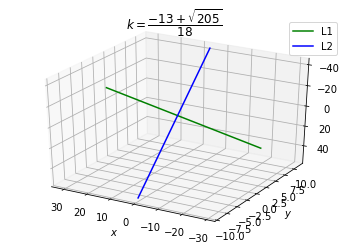
\includegraphics[width=\columnwidth]{Assignment4(1).png}
 \caption{Intersecting lines - Case1}
 \label{plot}
\end{figure}
\begin{figure}[!h]
 \centering
 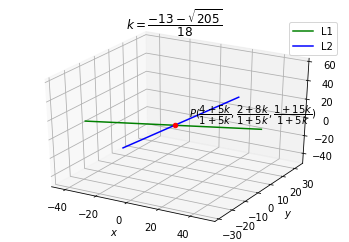
\includegraphics[width=\columnwidth]{Assignment4(2).png}
 \caption{Intersecting lines - Case2}
 \label{plot}
\end{figure}
\end{document}